% Intuition behind Bayesian Structural Time-Series Models
% author: Ivan Marevic

%% --- document settings --- %%
\documentclass{beamer}
\usetheme{Madrid}
\usecolortheme{beaver}
\usepackage[english]{babel}
\usepackage{eurosym}
\usepackage{graphicx}
\usepackage{amsmath}
\usepackage{xcolor}
\graphicspath{ {../plots/} }

% set toc settings
\definecolor{customred}{RGB}{161,22,22}
\setbeamertemplate{section in toc}[square]
\setbeamercolor{section number projected}{bg=customred,fg=white}
\setbeamertemplate{subsection in toc}{%
  \hspace{1.2em}{\color{customred}\rule[0.3ex]{3pt}{3pt}}~\inserttocsubsection\par}
\setbeamercolor*{item}{fg=customred}

% modify footer settings
\makeatletter
\setbeamertemplate{footline}{
  \leavevmode%
  \hbox{%
  \begin{beamercolorbox}[wd=.2\paperwidth,ht=2.25ex,dp=1ex,center]{author in head/foot}%
    \usebeamerfont{author in head/foot}\insertshortauthor\expandafter\ifblank\expandafter{\beamer@shortinstitute}{}{~~(\insertshortinstitute)}
  \end{beamercolorbox}%
  \begin{beamercolorbox}[wd=.5\paperwidth,ht=2.25ex,dp=1ex,center]{title in head/foot}%
    \usebeamerfont{title in head/foot}\insertshorttitle
  \end{beamercolorbox}%
  \begin{beamercolorbox}[wd=.3\paperwidth,ht=2.25ex,dp=1ex,right]{date in head/foot}%
    \usebeamerfont{date in head/foot}\insertshortdate{}\hspace*{2em}
    \insertframenumber{} / \inserttotalframenumber\hspace*{2ex} 
  \end{beamercolorbox}}%
  \vskip0pt%
}
\makeatother


%% --- start document --- %%
\begin{document}

\title{Intuition Behind Bayesian Structural Time-Series Models}   
\author{Ivan Marevic} 
\date{\today}

\begin{frame}
\titlepage
\end{frame}

\begin{frame}
\frametitle{Contents}\tableofcontents
\end{frame}


\section{Why Time-Series?} 
% What are time-series?
\begin{frame}[t]\frametitle{What are Time-Series?}
\begin{itemize}
\item A time-series is a sequence of observations taken sequentially in time
\item Goals of time-series modelling:
	\begin{itemize} 
	\item Understand stochastic mechanisms that give rise to the time-series
	\item Predict future trajectory of time-series
	\end{itemize}
\item Time-series can be \textit{univariate} or \textit{multivariate}:
\bigskip

\begin{tabular}{||c c||} 
 \hline
 Date &  Revenue \\ [0.5ex] 
 \hline\hline
 03.05.2020 & 845\euro \\ 
 \hline
 04.05.2020 & 756\euro \\
 \hline
 05.05.2020 & 545\euro \\
 \hline
 06.05.2020 & 834\euro \\
 \hline
 07.05.2020 & 957\euro \\
 \hline
\end{tabular}
\quad
\begin{tabular}{||c c c||} 
 \hline
 Date & Revenue & Weather \\ [0.5ex] 
 \hline\hline
 03.05.2020 & 845\euro & sunny \\ 
 \hline
 04.05.2020 & 756\euro & cloudy\\
 \hline
 05.05.2020 & 545\euro & rainy\\
 \hline
 06.05.2020 & 834\euro & rainy\\
 \hline
 07.05.2020 & 957\euro & sunny\\
 \hline
\end{tabular}

\end{itemize} 
\end{frame}

% time-series examples
\begin{frame}\frametitle{Time-Series Examples}
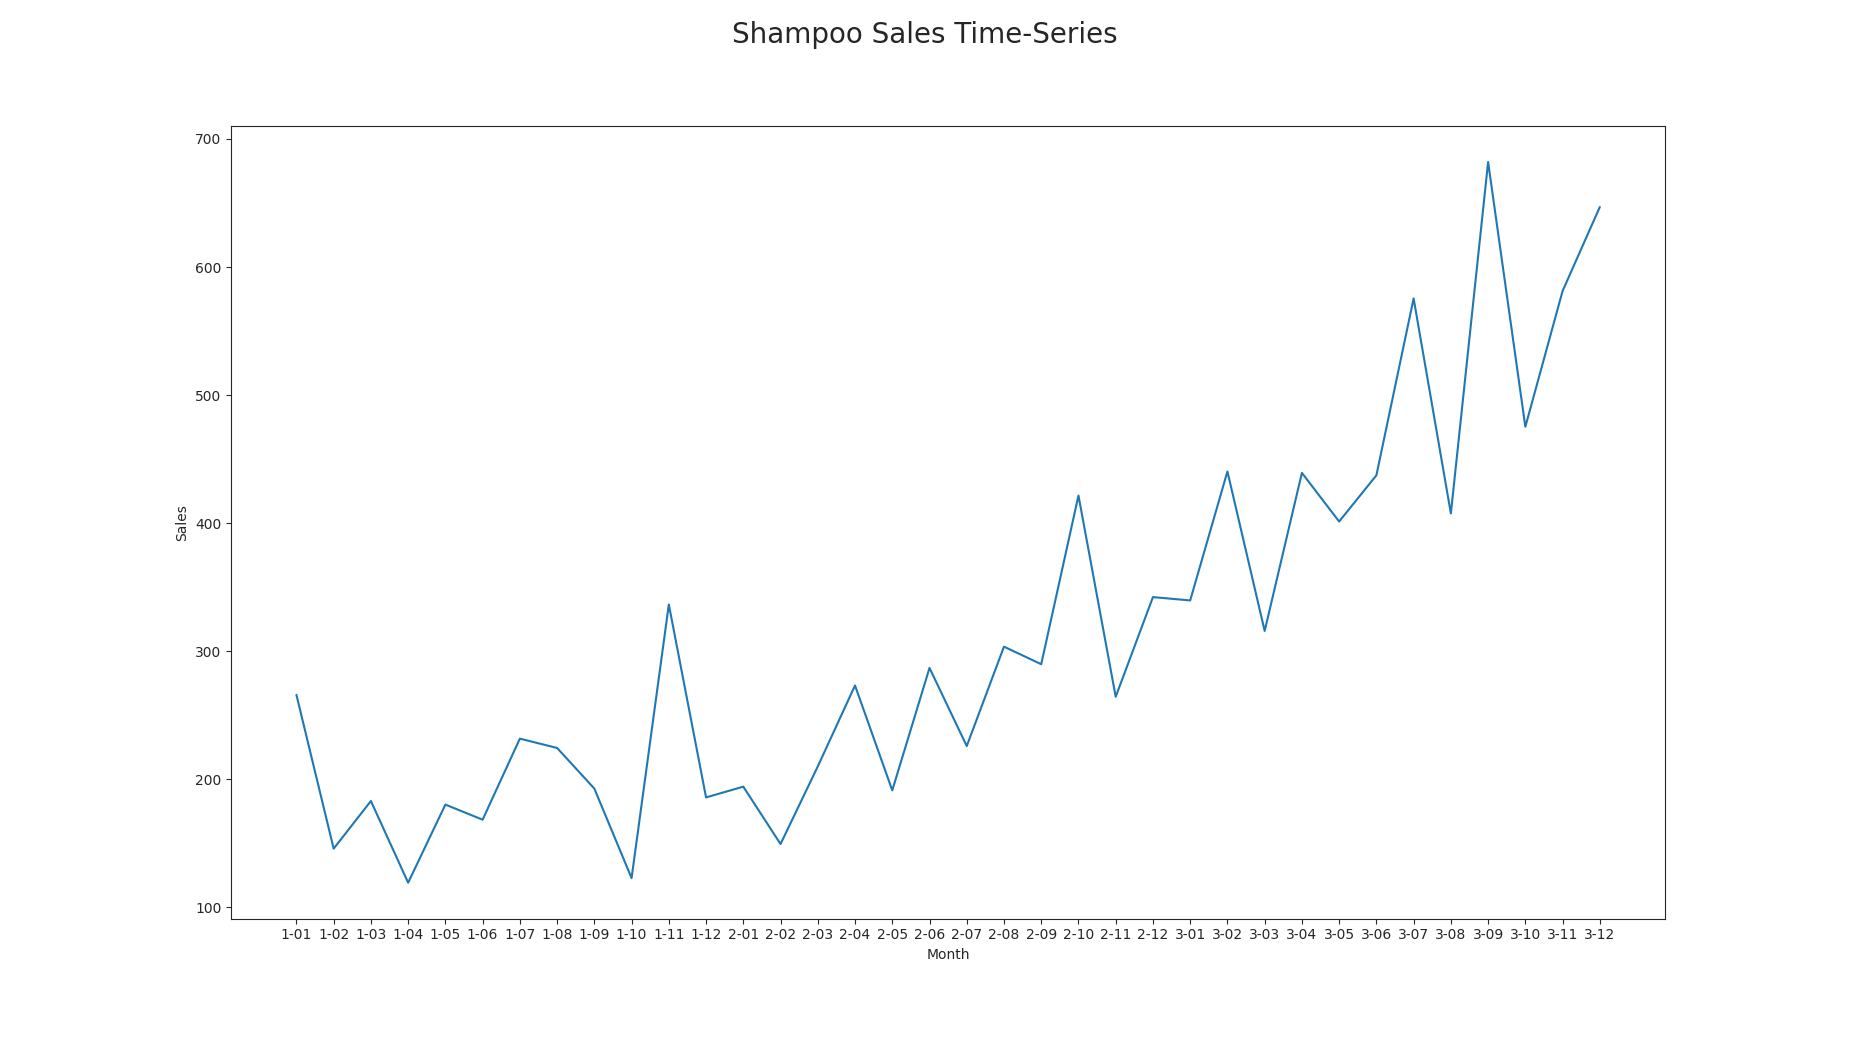
\includegraphics[width=\textwidth]{shampoo_ts}
\end{frame}

\begin{frame}\frametitle{Time-Series Examples}
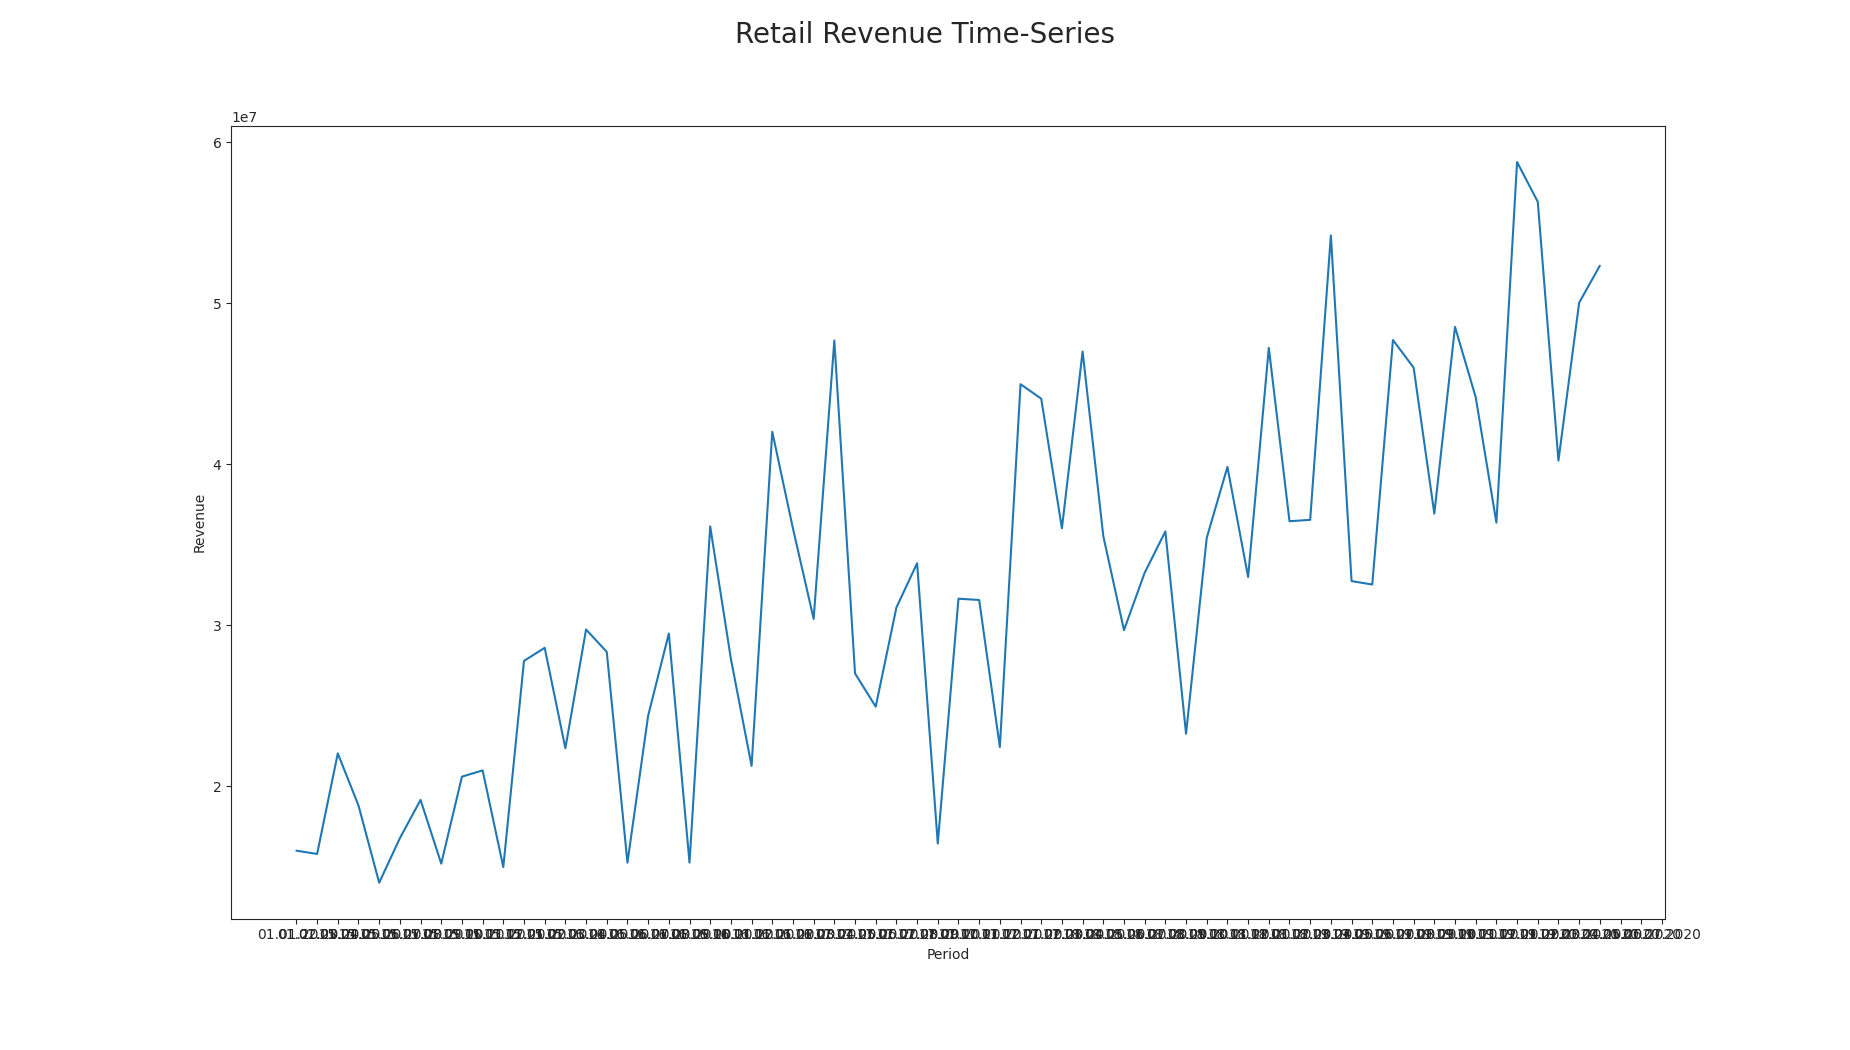
\includegraphics[width=\textwidth]{retail_revenue_ts}
\end{frame}

\begin{frame}\frametitle{Time-Series Examples}
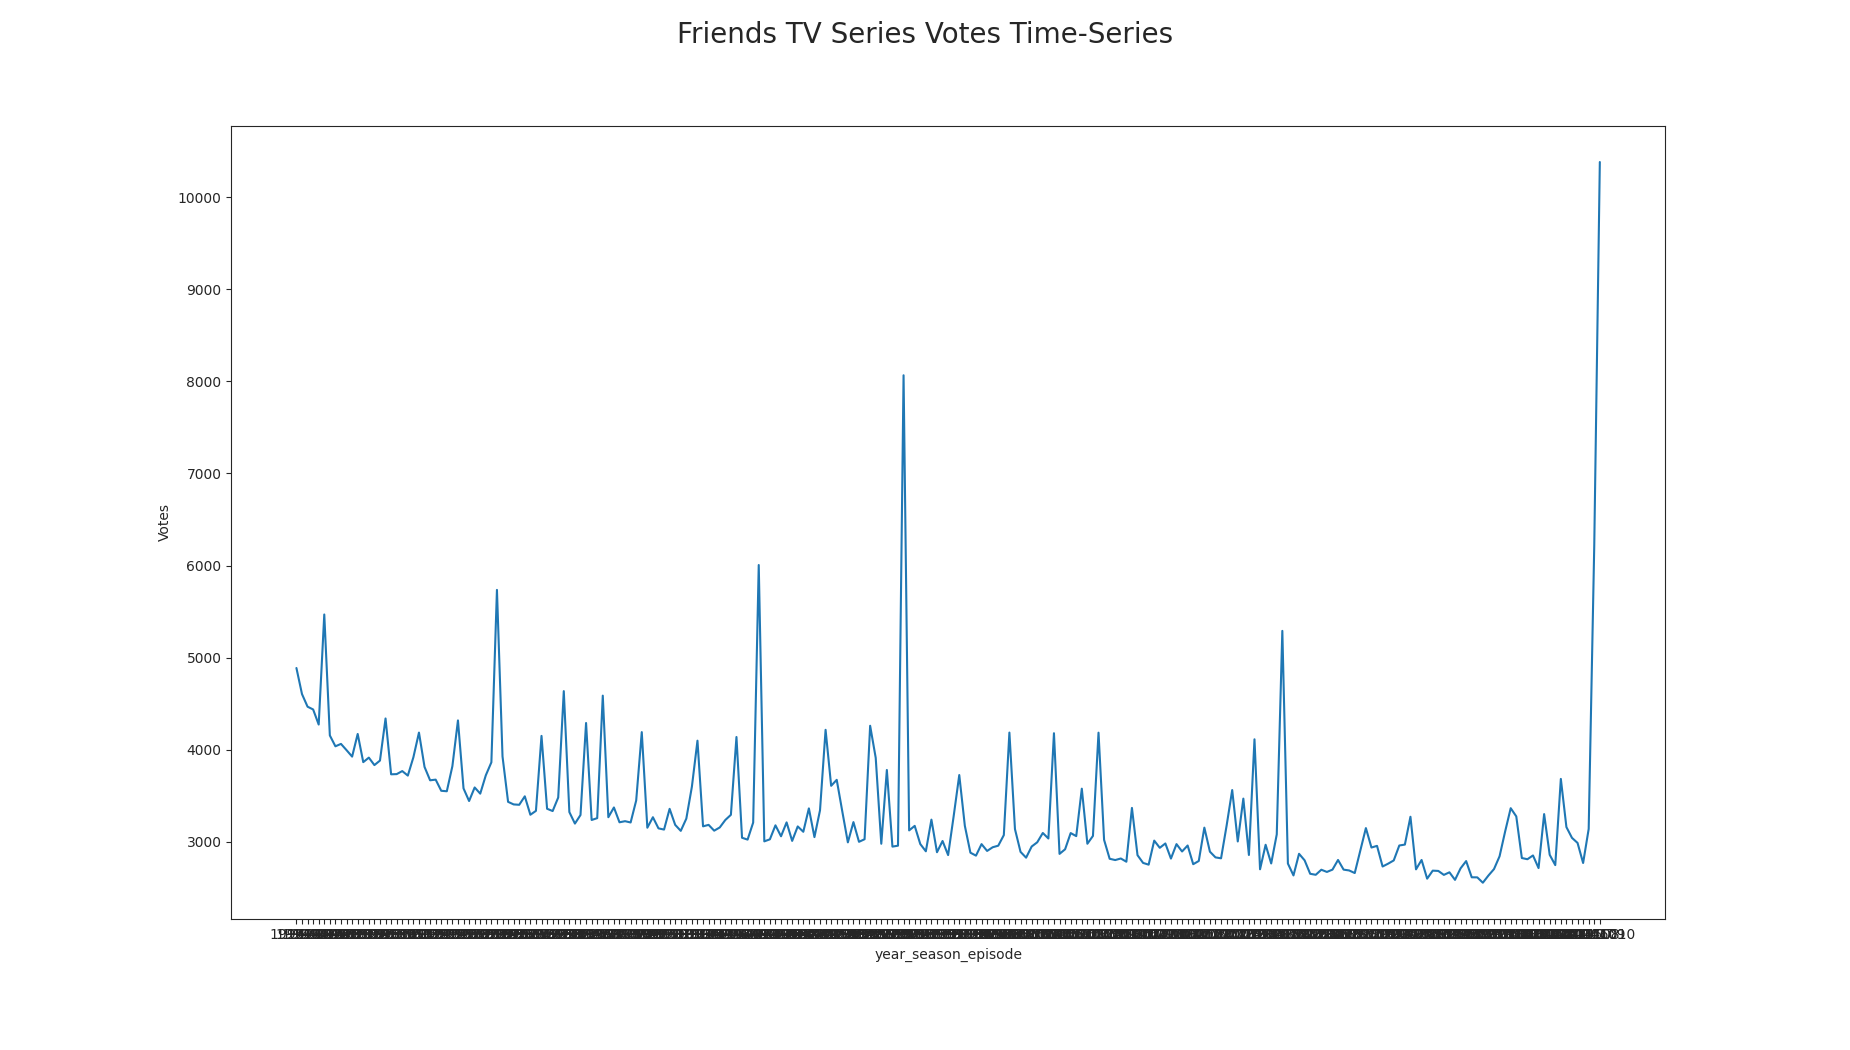
\includegraphics[width=\textwidth]{friends_episodes_votes_ts}
\end{frame}

\begin{frame}\frametitle{Time-Series Examples}
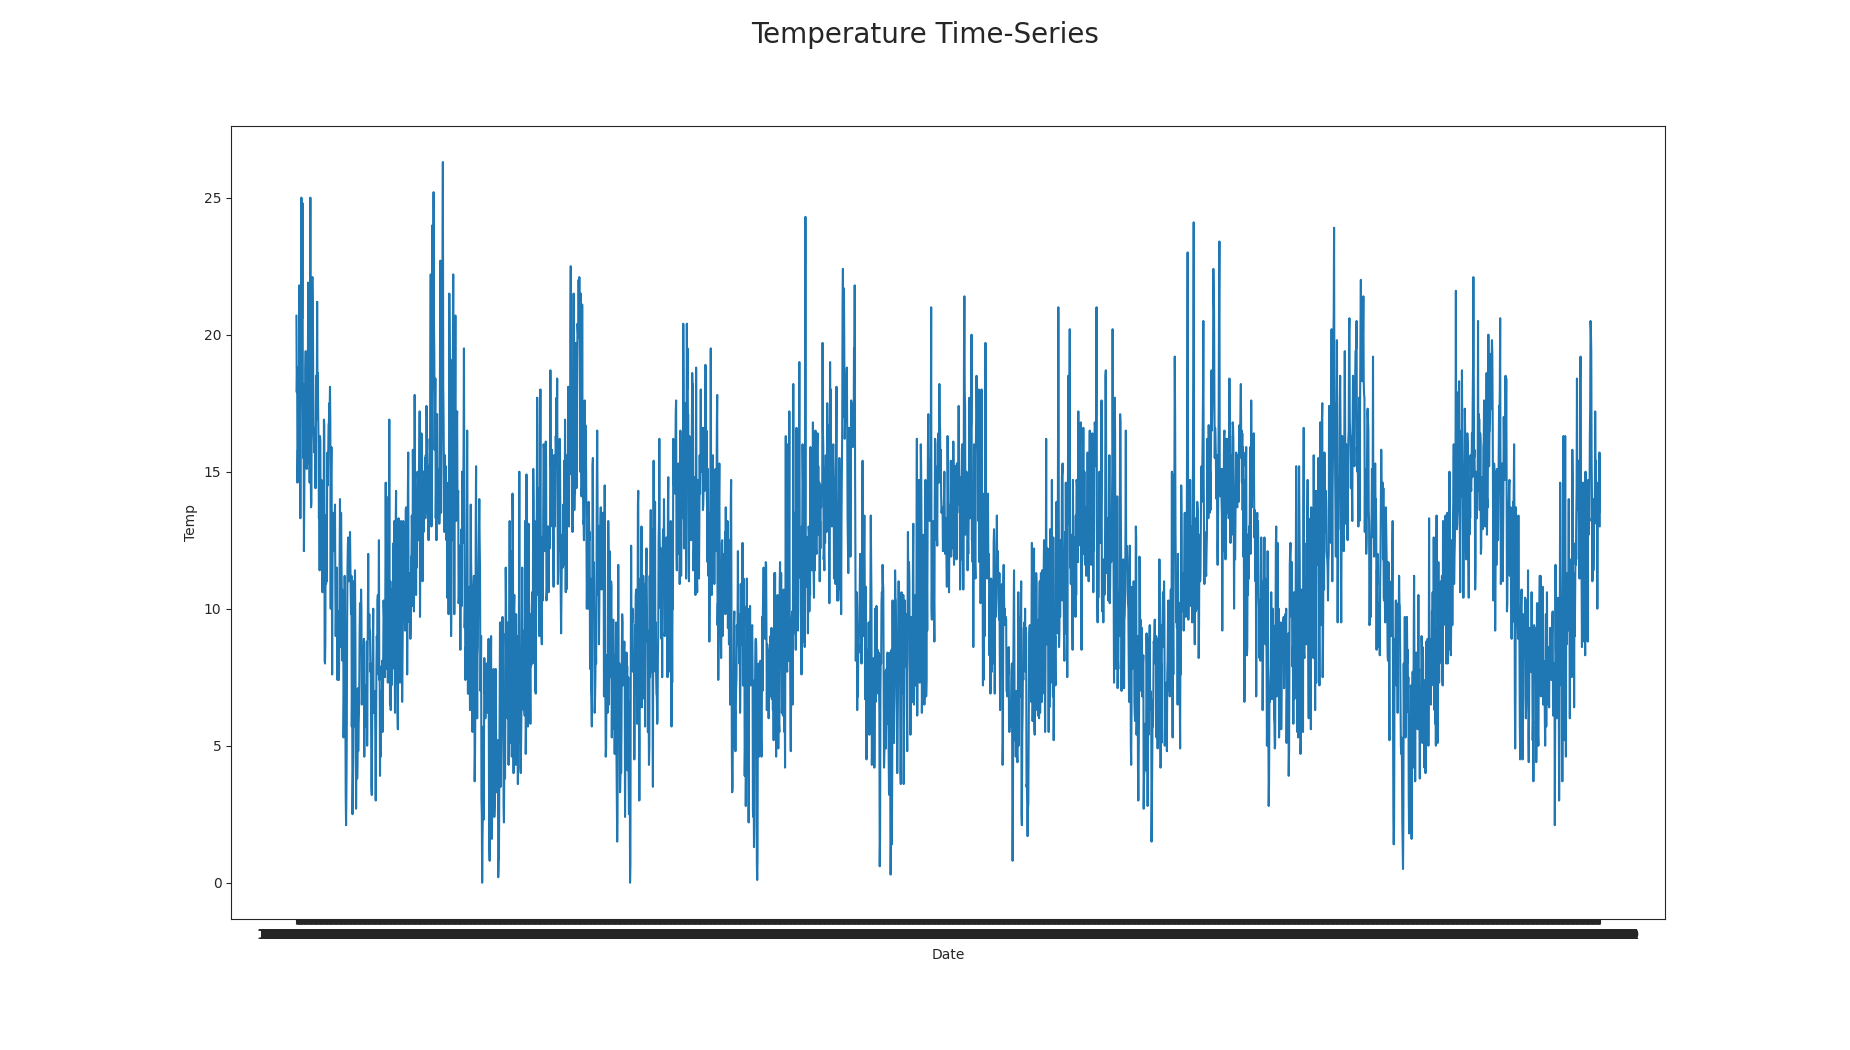
\includegraphics[width=\textwidth]{temperature_ts}
\end{frame}


\section{Unobserved Components Models} 
\subsection{UCM General Model Definition}
\begin{frame}[t]\frametitle{Unobserved Components Models}
\begin{itemize}
\item Time Series = Regression Effects + Trend + Cycles + Seasons + Irregularity-Term
\item Each component captures some important feature of the time-series
\item Components can have own probabilistic models (but can be modeled deterministically)
\item More components are possible depending on the use case
\item Traditional time-series model:\\
\bigskip
\[y_{t} = T_{t}+S_{t}+C_{t}+I_{t} \] \\
\bigskip
T = Trend;
S = Seasonal Component;
C = Cyclical Component;
I = Irregular Component
\end{itemize} 
\end{frame}

\begin{frame}[t]\frametitle{Unobserved Components Models}
Fully specified UC Model:
\bigskip
\[y_{t} = \mu_{t}+\gamma_{t}+\psi_{t}+r_{t}+\sum_{i=1}^p\phi_{i}y_{t-i} + \sum_{j=1}^m\beta_{j}x_{jt}+\varepsilon_{t}  \] \\
\bigskip
\begin{itemize}
\item $y_{t}$: time-series to be modeled\\ 
\item $\mu_{t}$: time varying mean (trend component)\\
\item $\gamma_{t}$: seasonal component\\
\item $\psi_{t}$: cyclical component\\
\item $r_{t}$: autoregressive component\\
\item $\sum_{i=1}^p\phi_{i}y_{t-i}$: momentum of time-series with respect to past timepoints\\
\item $\sum_{j=1}^m\beta_{j}x_{jt}$: additional predictors\\
\item $\varepsilon_{t}$: irregular component (error term)
\end{itemize}
\end{frame}


\begin{frame}[t]\frametitle{UCM Deterministic Example}
Considering a traditional UC time-series, we can construct a deterministic example:
\bigskip
\begin{align*}
y_{t} &= \color{blue}T_{t}
	   \color{black}+ \color{orange} C_{t}
	   \color{black}+ \color{violet} S_{t}
	   \color{black}+ \color{red} I_{t} \\
	  &= \color{blue} 100+4t \\
	  &+ \color{orange} 50*cos(\pi t/10) \\
	  &- \color{violet} 50jan-25feb+25mar-25apr-50may+50jun \\
	  &+ \color{violet} 75jul+50aug+5sep-25oct-50nov+20dec \\
	  &+ \color{red} \varepsilon_{t}
\end{align*}
\begin{itemize}
\item jan, feb, ..., dec $\Rightarrow$ 1 if \textit{t} in respective month, else 0
\item $\varepsilon_{t} \sim \mathcal{N}(\mu,\,\sigma^{2})$ with $\mu = 0; \sigma^{2} = 10$

\end{itemize}
\end{frame}

\begin{frame}[t]\frametitle{UCM Deterministic Example - Trend}
Modeling linear trend (\textit{T}): \\
\[T_{t} = 100+4t\]
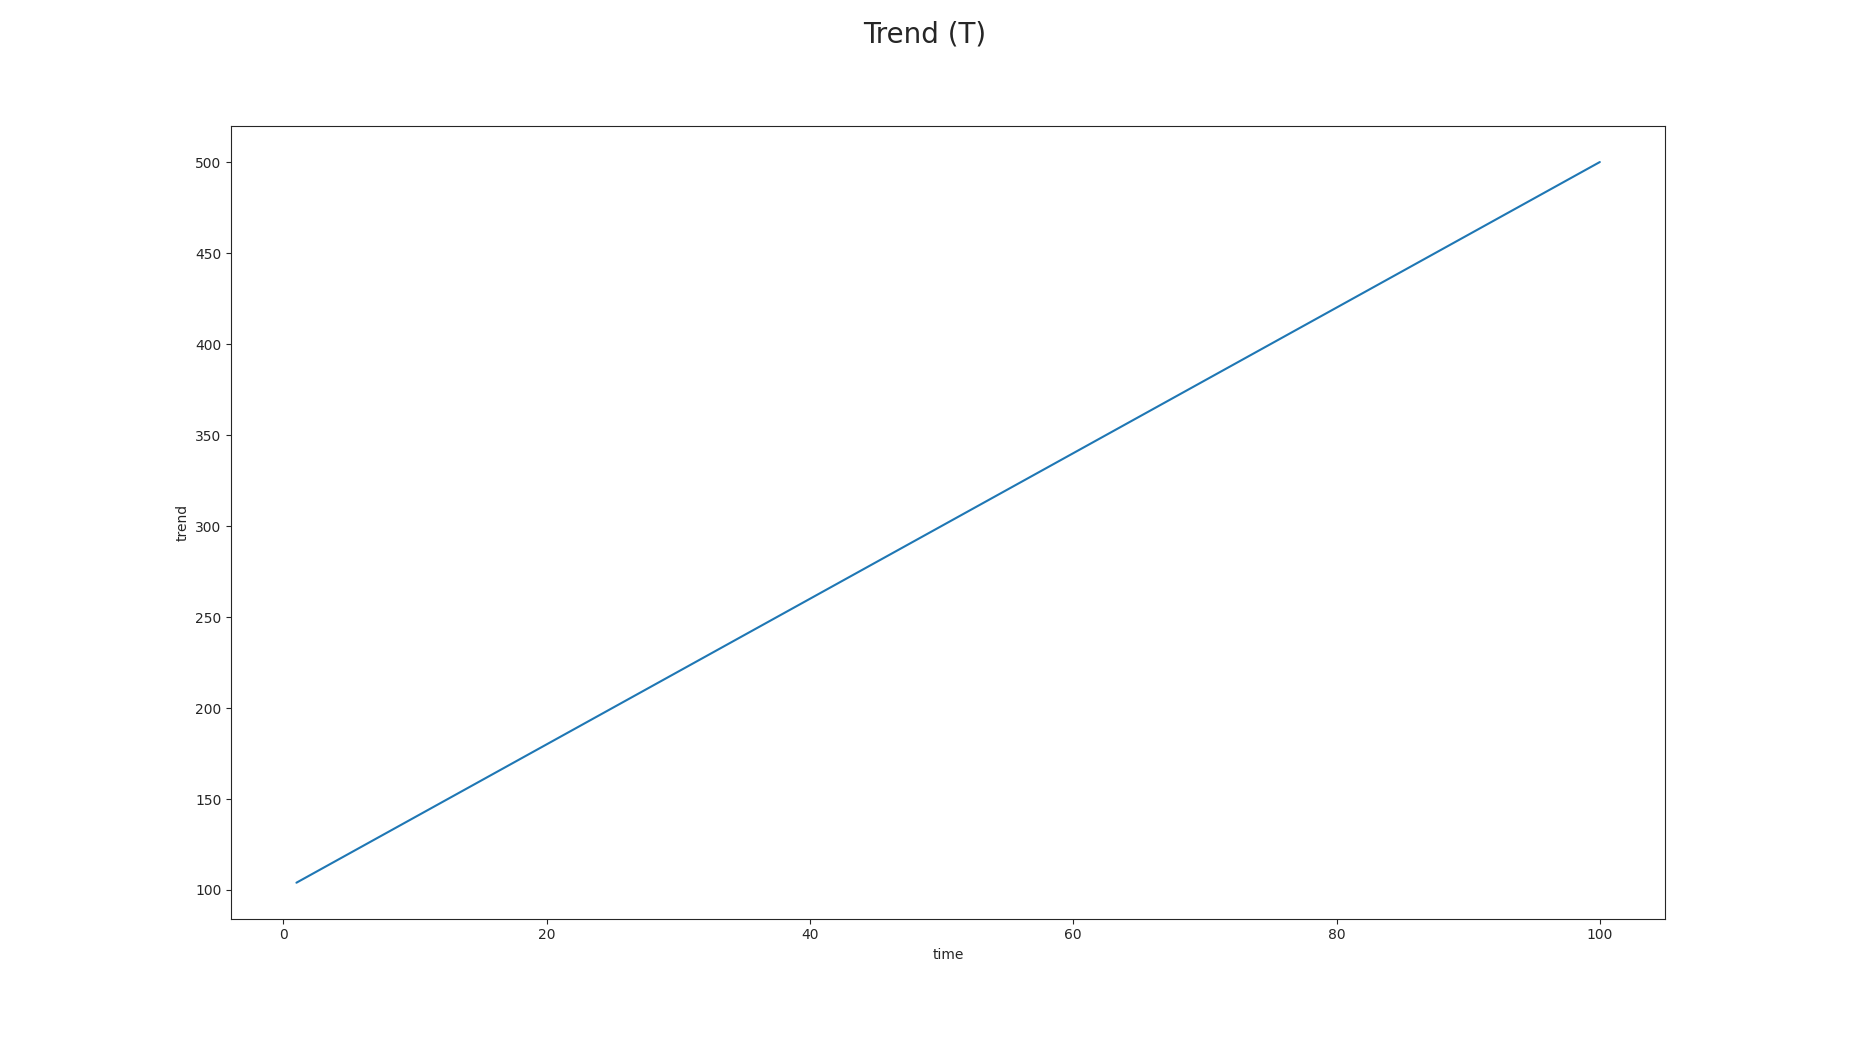
\includegraphics[width=\textwidth, height=0.7\textheight]{ucm_deterministic_trend}
\end{frame}

\begin{frame}[t]\frametitle{UCM Deterministic Example - Cyclical Component}
Modeling cyclicality (\textit{C}): \\
\[C_{t} = 50*cos(\pi t/10)\]
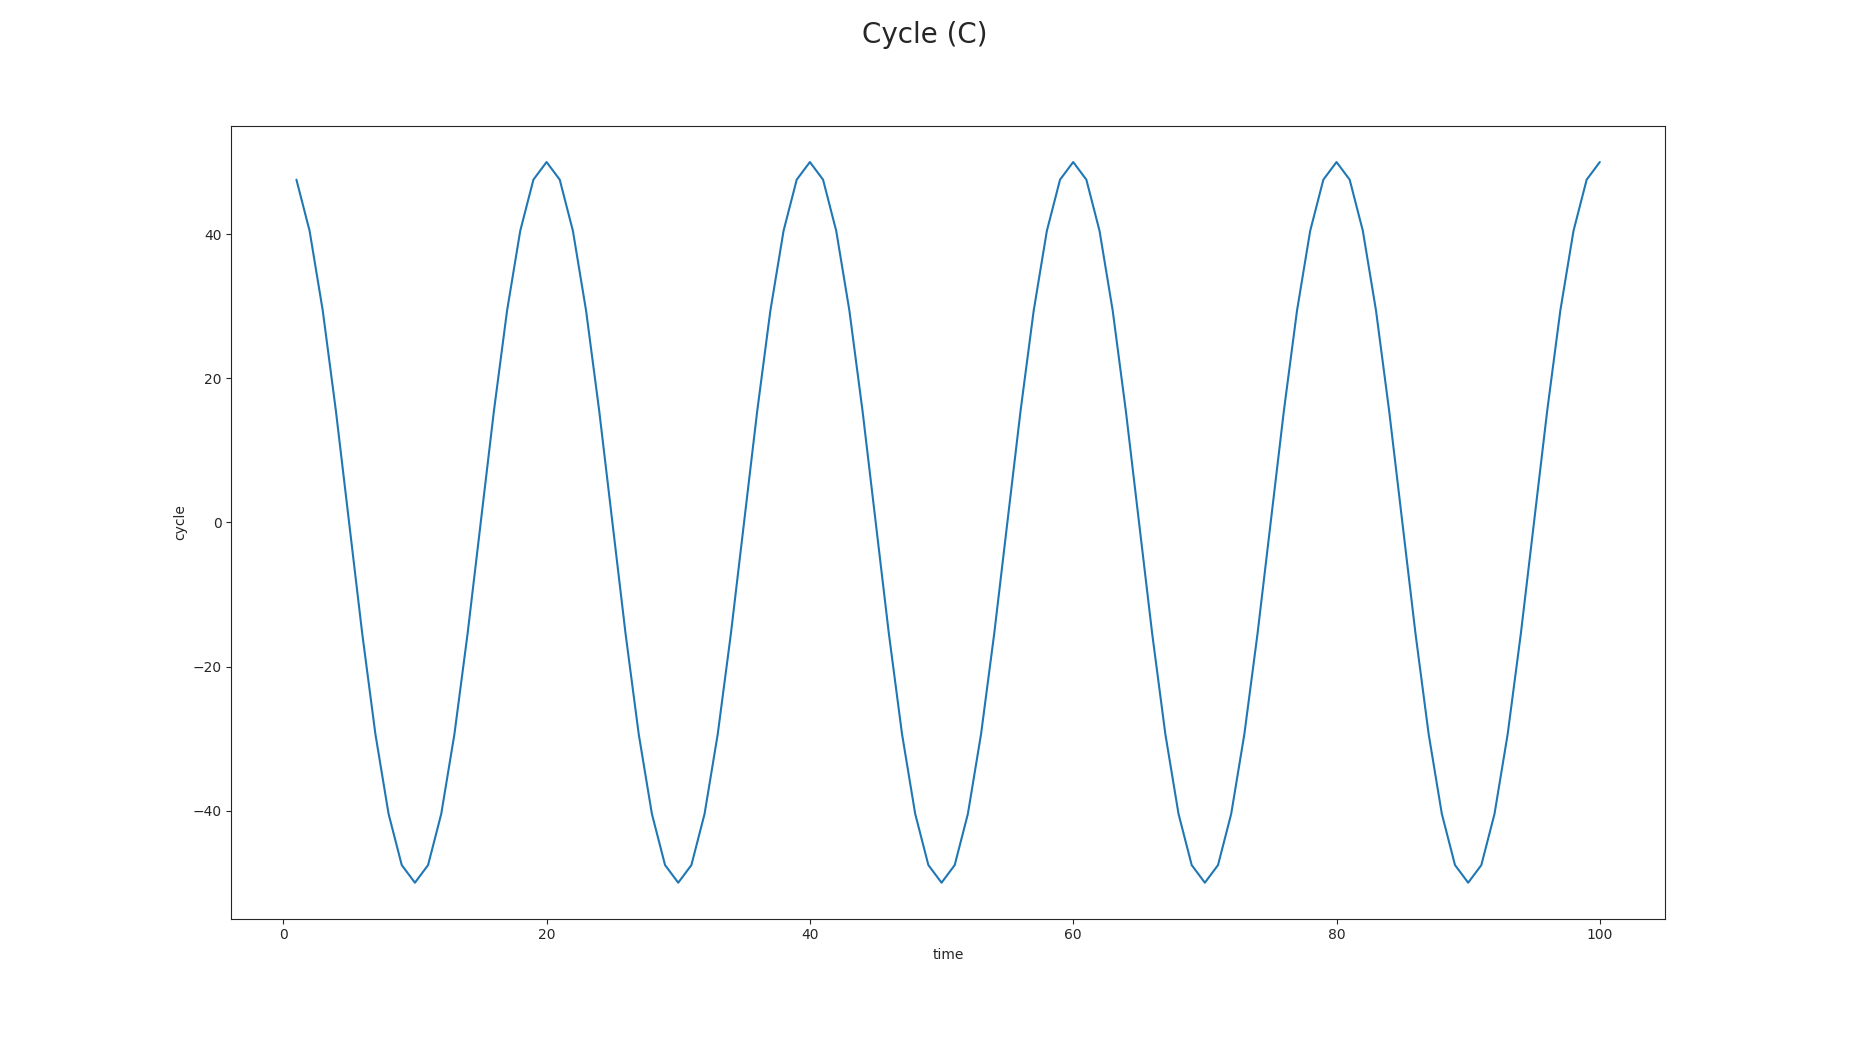
\includegraphics[width=\textwidth, height=0.7\textheight]{ucm_deterministic_cycle}
\end{frame}

\begin{frame}[t]\frametitle{UCM Deterministic Example - Seasonal Component}
Modeling seasonality (\textit{S}): \\
\begin{align*}
S_{t} = &-50jan-25feb+25mar-25apr-50may+50jun \\
&+75jul+50aug+5sep-25oct-50nov+20dec
\end{align*}
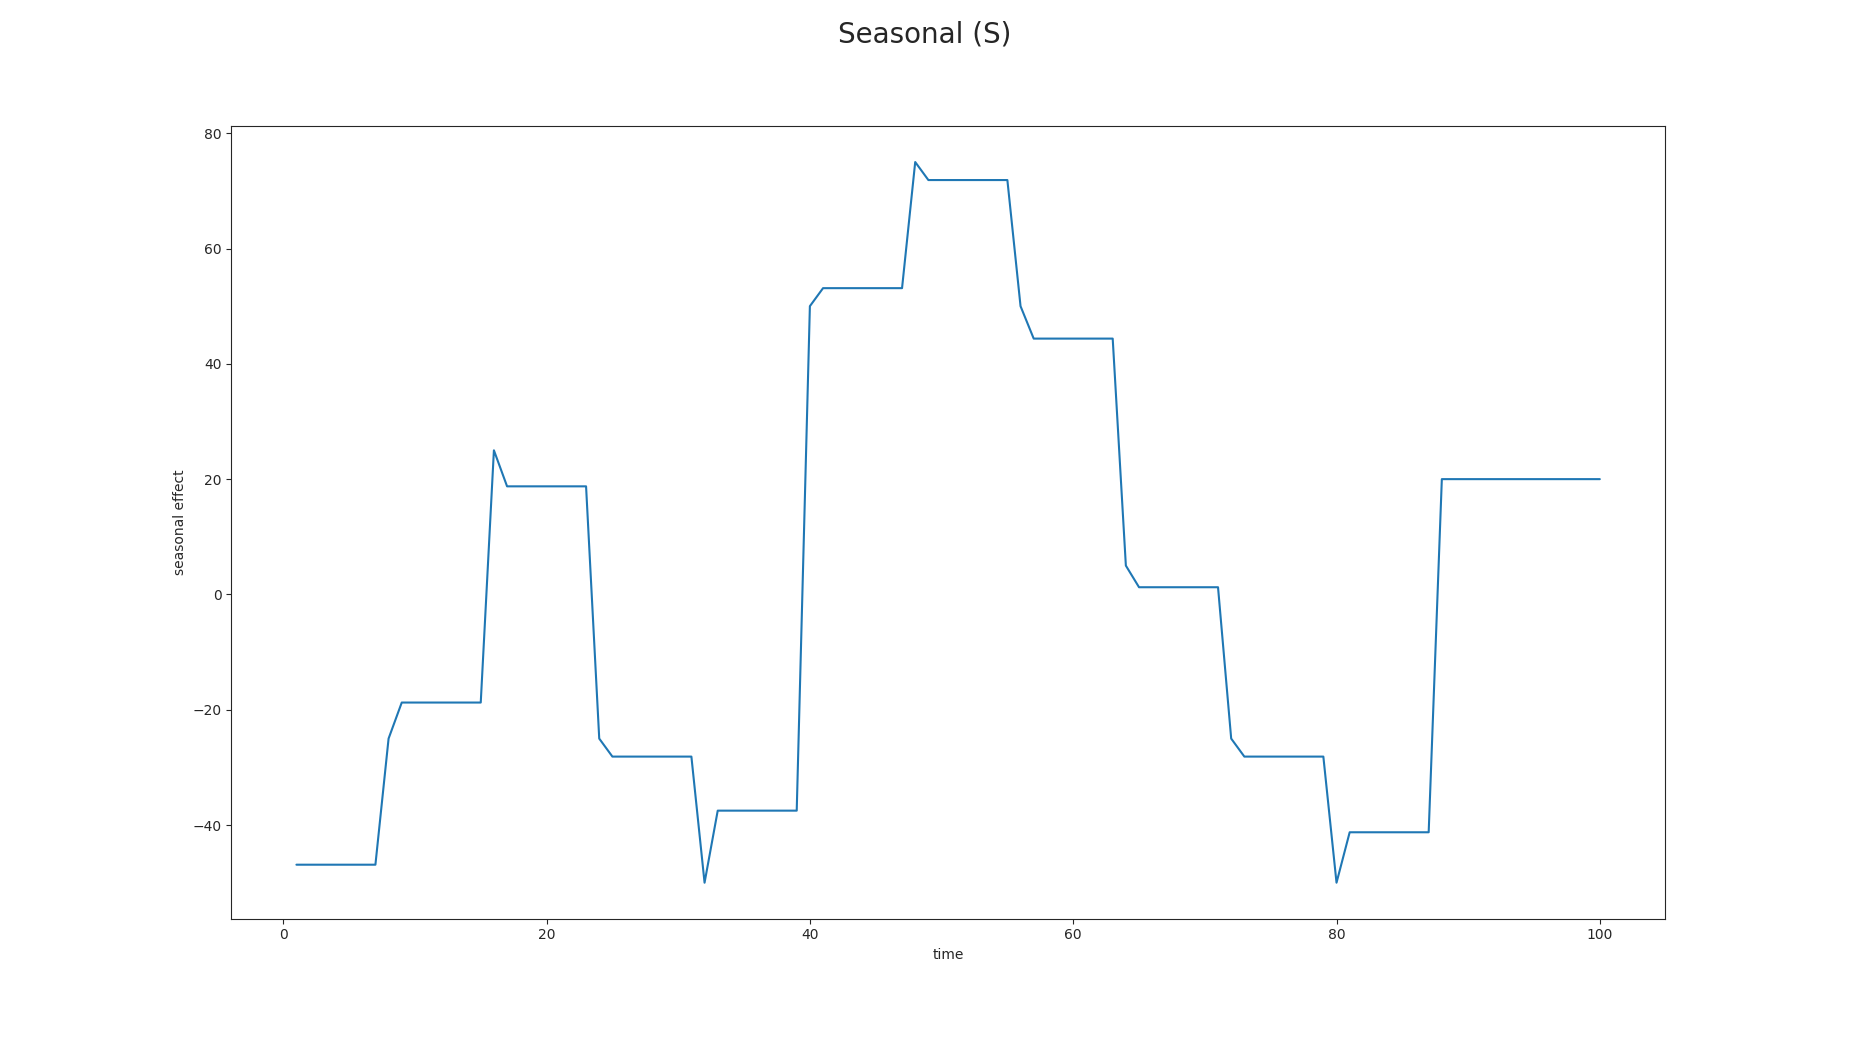
\includegraphics[width=\textwidth, height=0.6\textheight]{ucm_deterministic_seasonal}
\end{frame}

\begin{frame}[t]\frametitle{UCM Deterministic Example - Irregular Component}
Modeling irregularity (\textit{I}): \\
\[I_{t} = \varepsilon_{t} \sim \mathcal{N}(\mu,\,\sigma^{2});  \mu = 0; \sigma^{2} = 10 \]
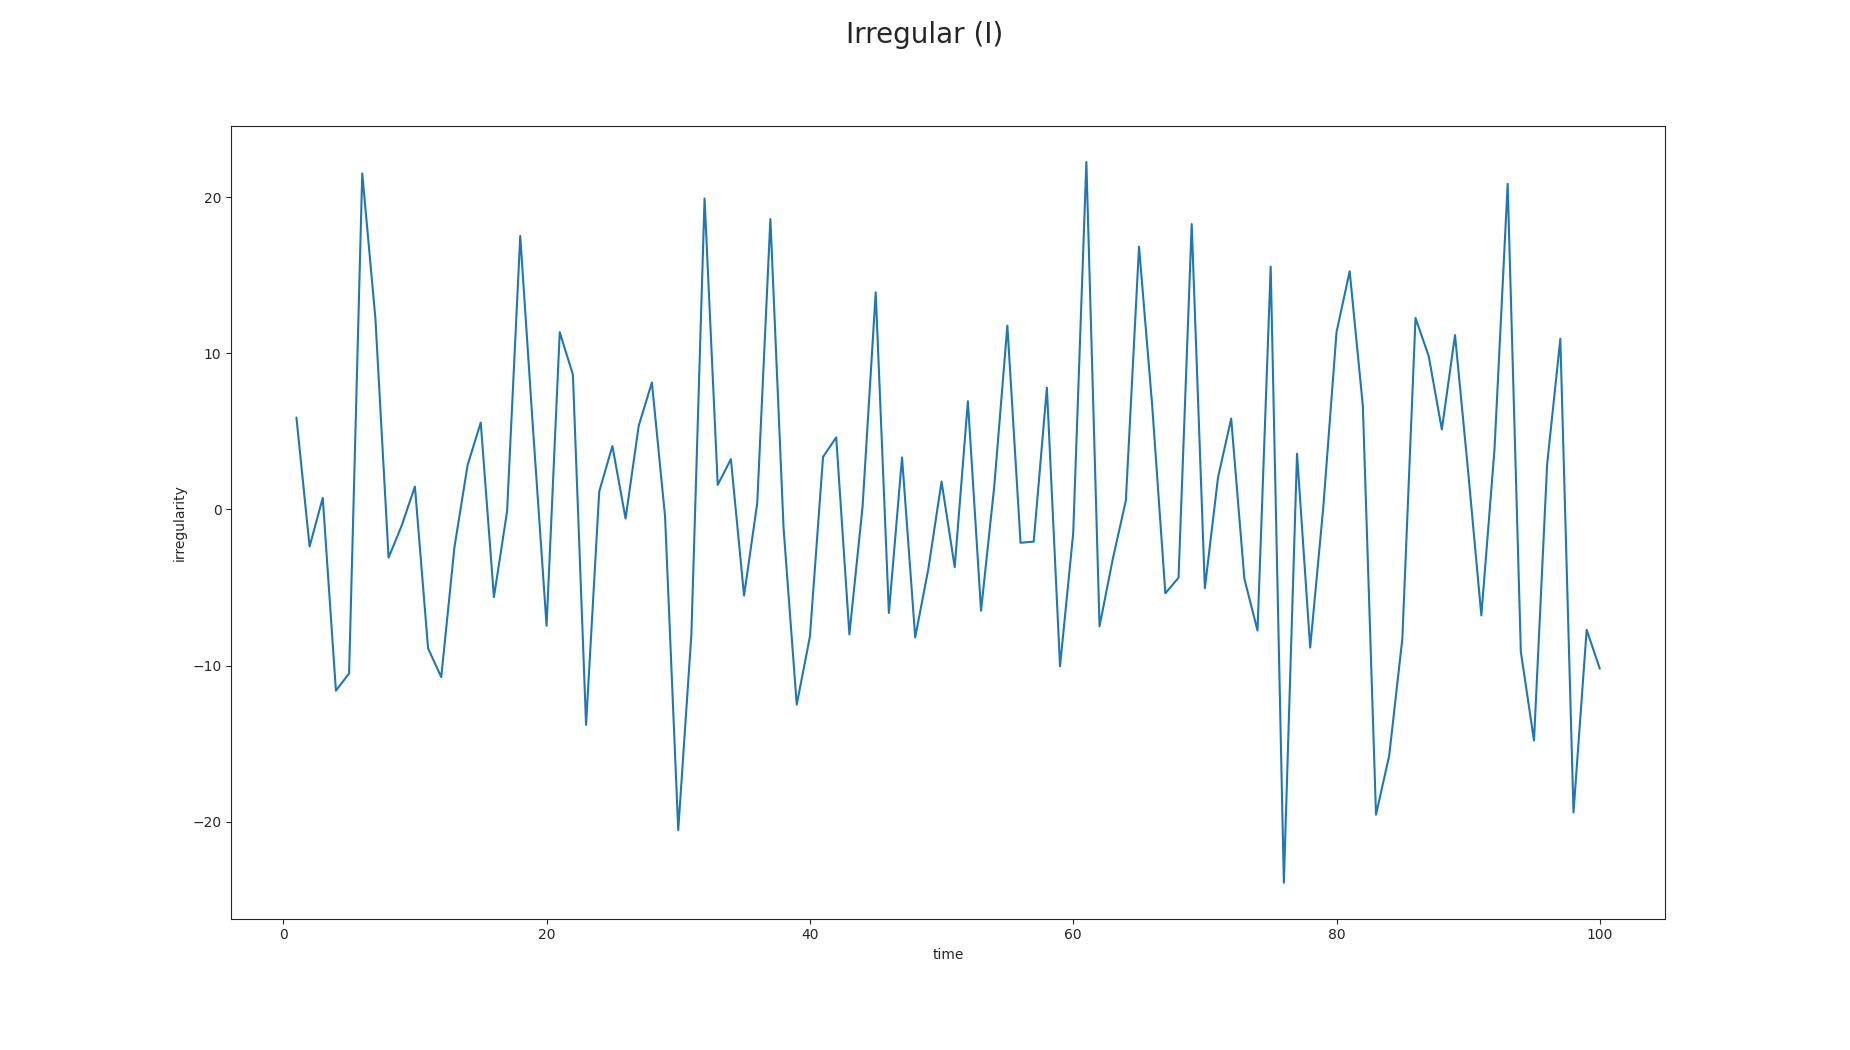
\includegraphics[width=\textwidth, height=0.7\textheight]{ucm_deterministic_irregular}
\end{frame}

\begin{frame}[t]\frametitle{UCM Deterministic Example: T + C}
\[y_{t} = T_{t}+C_{t}\]
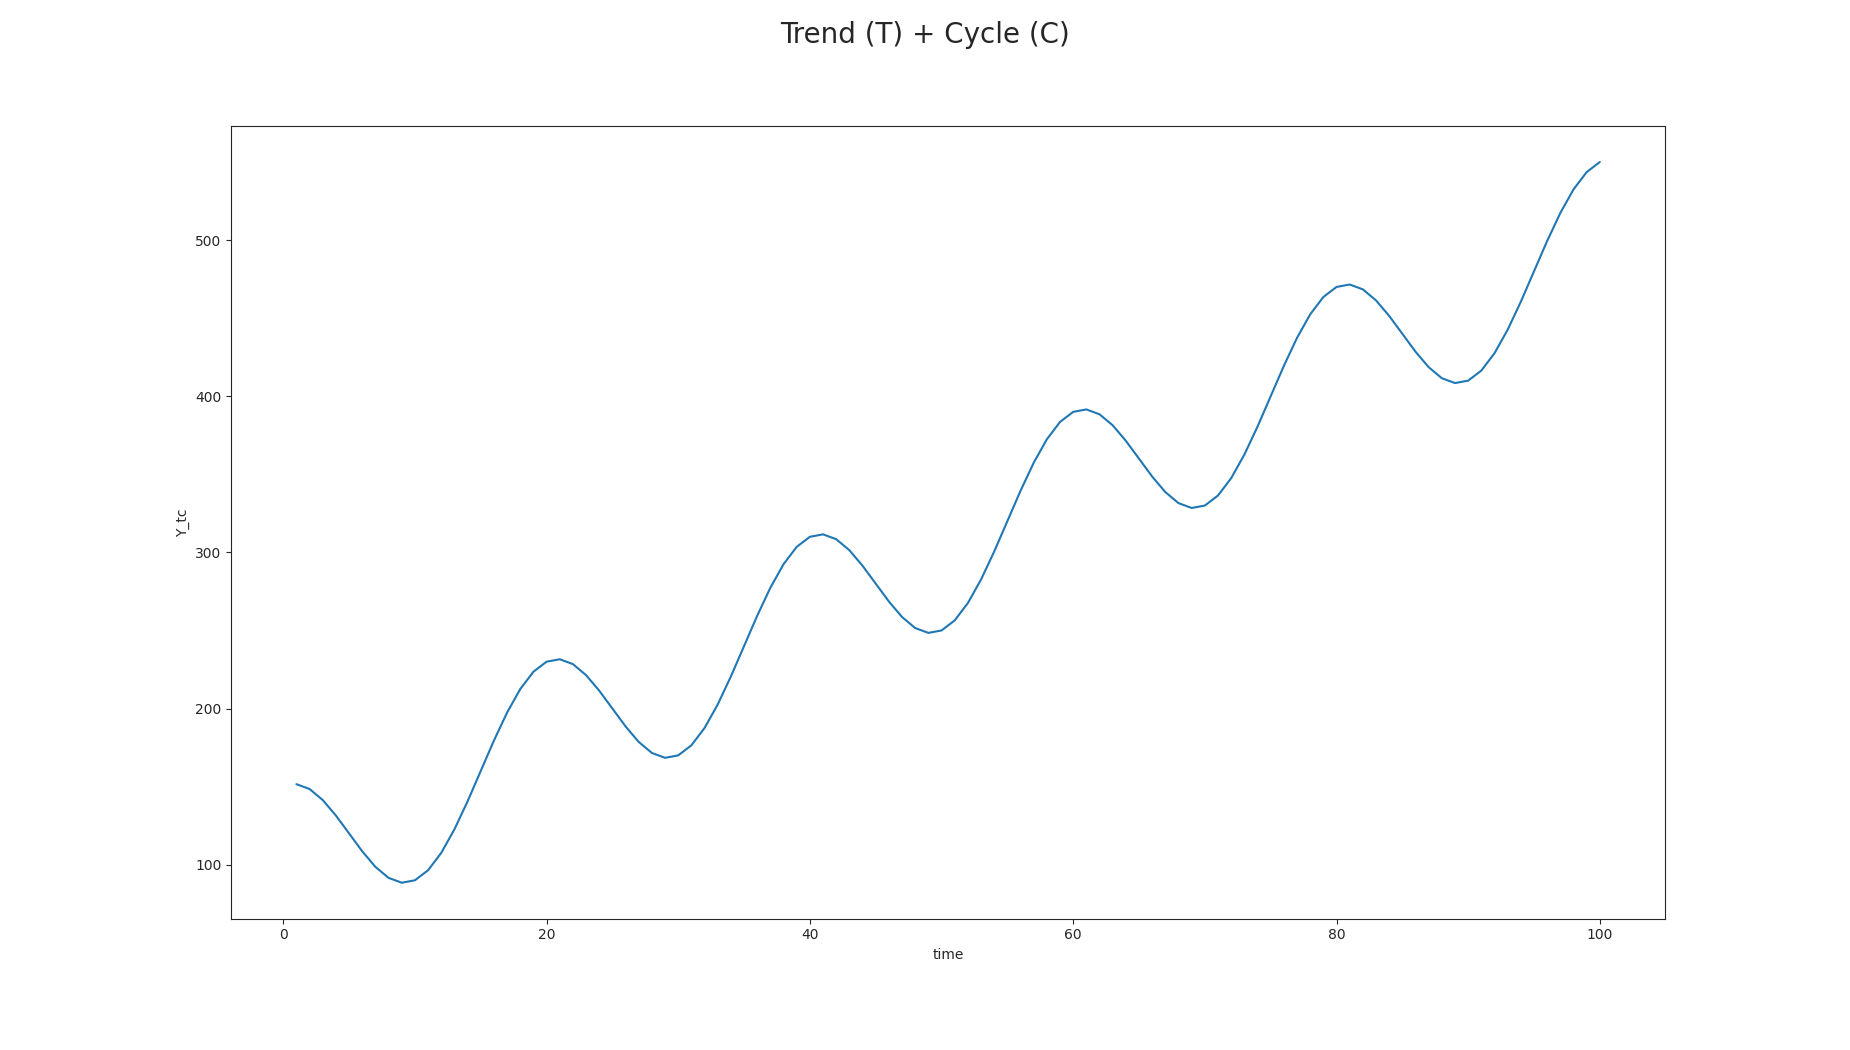
\includegraphics[width=\textwidth, height=0.7\textheight]{ucm_deterministic_trend_cycle}
\end{frame}

\begin{frame}[t]\frametitle{UCM Deterministic Example: T + C + S}
\[y_{t} = T_{t}+C_{t}+S_{t}\]
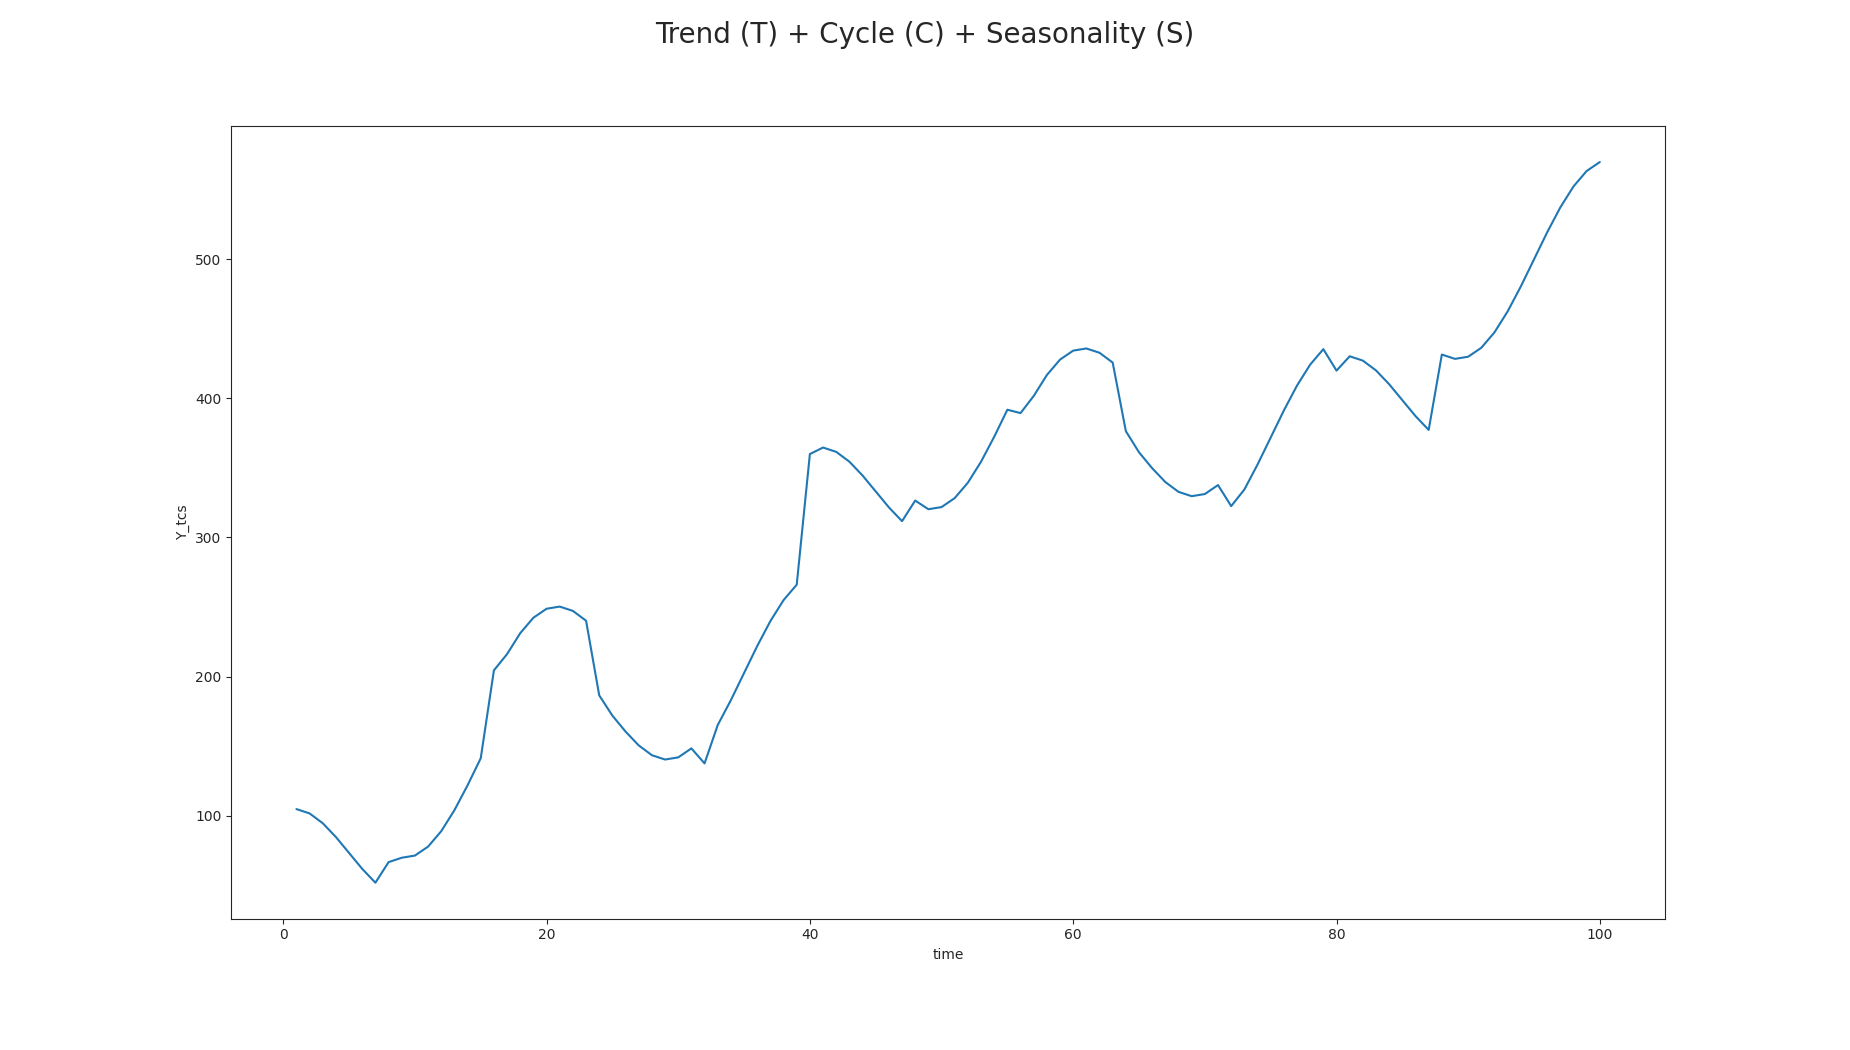
\includegraphics[width=\textwidth, height=0.7\textheight]{ucm_deterministic_trend_cycle_season}
\end{frame}

\begin{frame}[t]\frametitle{UCM Deterministic Example: T + C + S + I}
\[y_{t} = T_{t}+C_{t}+S_{t}+I_{t}\]
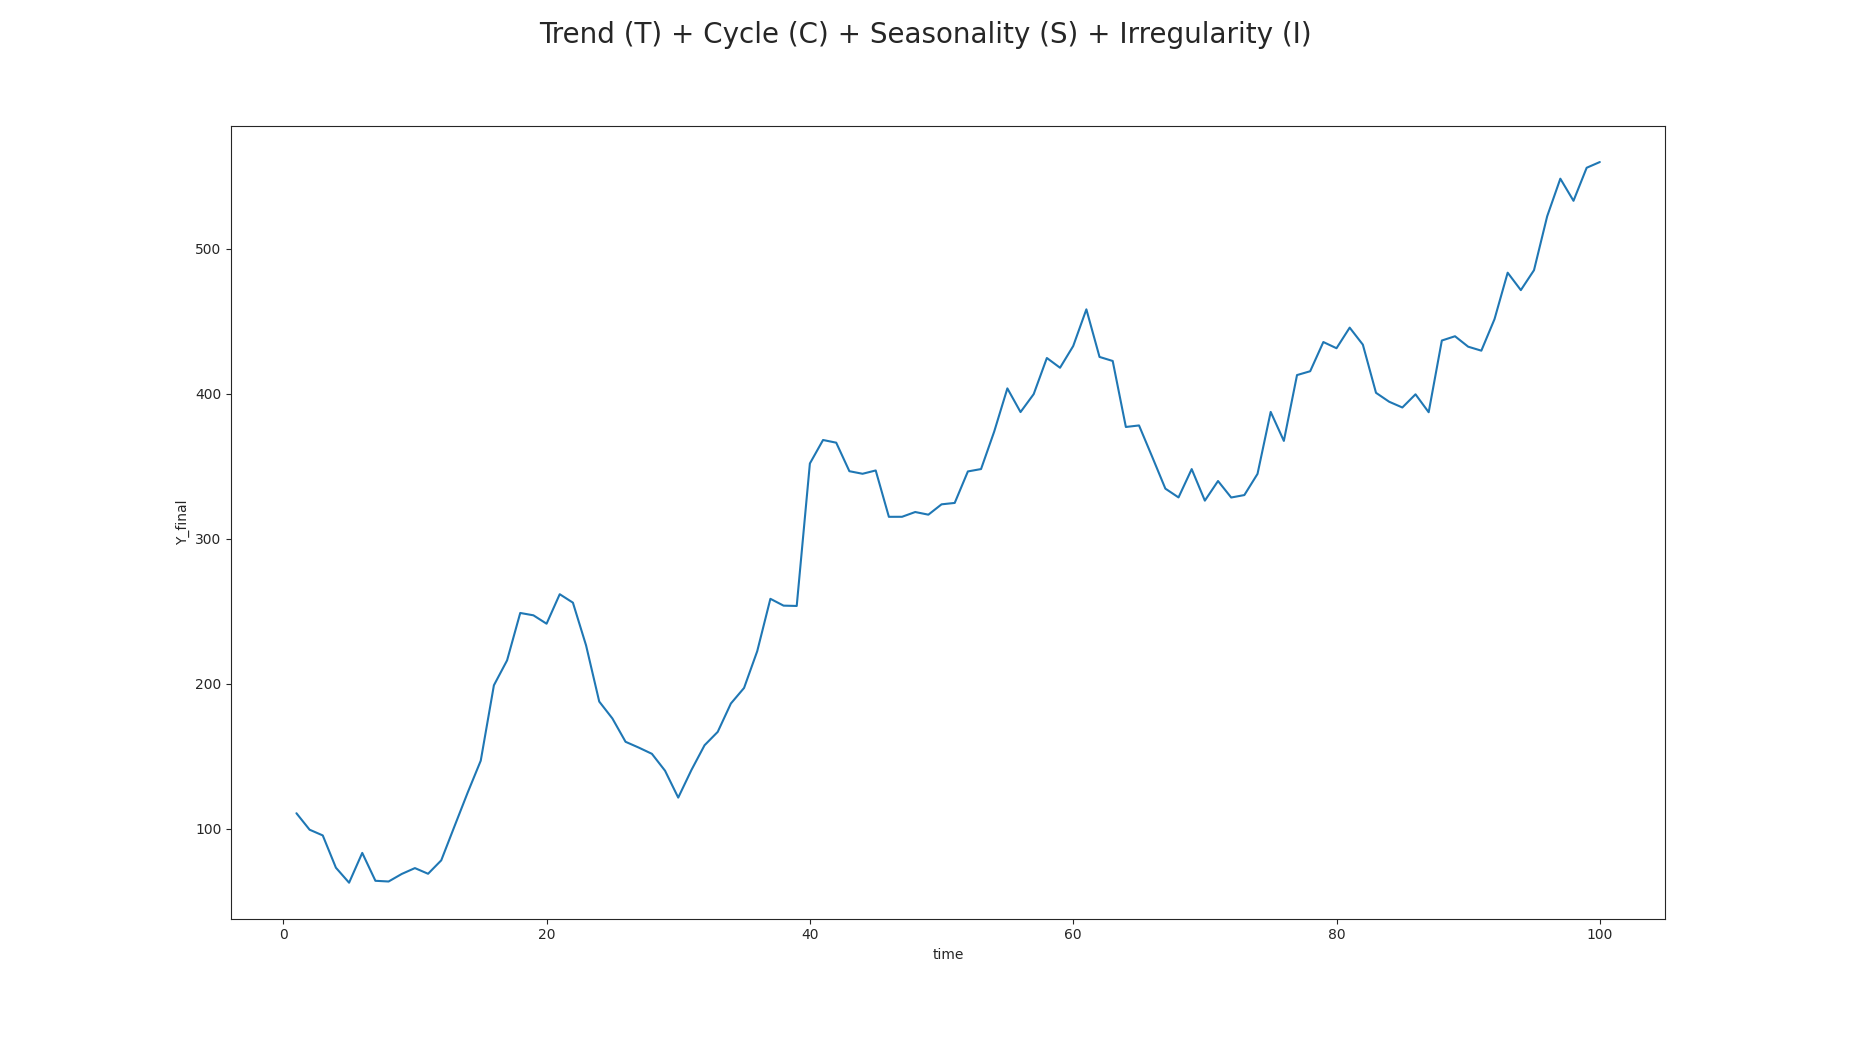
\includegraphics[width=\textwidth, height=0.7\textheight]{ucm_deterministic_full_model}
\end{frame}

\begin{frame}[t]\frametitle{Local Linear Trend (LLT)}
\begin{itemize}
\item Trend can also be modeled stochastically as a local linear trend (LLT)
\end{itemize}
\bigskip
\hspace{30pt} $\mu_{t} = \mu_{t-1} + \eta_{t-1} + \nu_{t}$ \hspace{30pt} level equation \\
\hspace{30pt} $\eta_{t} = \eta_{t-1} + \xi_{t}$ \hspace{67pt} slope equation
\bigskip
\begin{itemize}
\item disturbances in the level equation modeled as $\nu_{t} \sim \mathcal{N}(0,\,\sigma^{2}_{\nu})$
\item disturbances in the slope equation modeled as $\xi_{t} \sim \mathcal{N}(0,\,\sigma^{2}_{\xi})$
\item $\mu_{t}$ and $\eta_{t}$ can be initialized as unknown or random vectors
\end{itemize}
\bigskip
LLT in vector recursion form: \\
\begin{equation*}
\begin{pmatrix}
\mu_{t}\\
 \eta_{t}
\end{pmatrix}
=
\begin{pmatrix}
1 & 1\\
0 & 1
\end{pmatrix}
\begin{pmatrix}
\mu_{t-1}\\
 \eta_{t-1}
\end{pmatrix}
+
\begin{pmatrix}
\nu_{t}\\
 \xi_{t}
\end{pmatrix}
\end{equation*}
\end{frame}

\begin{frame}[t]\frametitle{LLT - Special Cases}
\begin{itemize}
\item Special cases of LLT can be constructed via elimination of specific parts
\item Deterministic examples are special cases of LLT
\end{itemize}
\begin{table}
\centering
\begin{tabular}{||c c||} 
 \hline
 \textit{model} &  \textit{description} \\ [0.5ex] 
 \hline\hline
 $\mu_{t} = \mu_{t-1} + \nu_{t}$ & initial slope and its disturbance = 0 \\ 
 \hline
 $\mu_{t} =  \mu_{t-1} + \eta_{1} +\nu_{t}$ & slope disturbance = 0  \\
 \hline
 $\mu_{t} =  \mu_{t-1} + \eta_{t-1}$; $\eta_{t} = \eta_{t-1} + \xi_{t}$ & level disturbance = 0  \\
 \hline
 $\mu_{t} = \mu_{1} + t\eta_{1}$ & deterministic time trend \\
 \hline
 $\mu_{ŧ} = \mu_{1}$ & degenerate time invariant \\
 \hline
\end{tabular}
\end{table}
\end{frame}

\begin{frame}[t]\frametitle{Cycles}
\begin{itemize}
\item Stochastic cycle can be modeled using recursion
\item For \textit{t} = 1,2,3,..., and $0<\omega<\pi$; \\
$\psi_{t} = \gamma\cos(\omega\textit{t} - \phi)$, $\gamma=\sqrt{a^2 + b^2}$, $\phi = \arctan(\textit{b}/\textit{a})$; and \\
$0 \leq \rho \leq 1; \nu_{t} \sim \mathcal{N}(0,\,\sigma^{2}_{\nu})$ and $\nu^*_{t} \sim \mathcal{N}(0,\,\sigma^{2}_{\nu})$
\end{itemize}
\bigskip
\begin{equation*}
\begin{pmatrix}
\psi_{t}\\
\psi^*_{t}
\end{pmatrix}
=
\rho
\begin{pmatrix}
\cos(\omega) & \sin(\omega)\\
-\sin(\omega) & \cos(\omega)
\end{pmatrix}
\begin{pmatrix}
\psi_{t-1}\\
\psi^*_{t-1}
\end{pmatrix}
+
\begin{pmatrix}
\nu_{t}\\
\nu^*_{t}
\end{pmatrix}
\end{equation*}
\begin{itemize}
\item resulting sequence $\psi_{t}$ is pseudo-cyclical with time-varying amplitude, phase, and period
\end{itemize}
\end{frame}


\begin{frame}[t]\frametitle{Seasons}
\begin{itemize}
\item Seasons are corrections to general trend of the time-series
\item Seasonal effects sum to 0 over one full season cycle
\item Two popular representations of seasonal patterns:
\end{itemize}
\begin{table}
\centering
\begin{tabular}{||p{0.45\linewidth} | p{0.45\linewidth}||}
 \hline
 \textit{Stochastic Dummy Type} &  \textit{Stochastic Trigonometric Type} \\ [0.5ex] 
 \hline\hline
 $\sum_{i=0}^{s-1} \gamma_{t-i} = \nu_{t}, \nu_{t} \sim \mathcal{N}(0,\sigma^{2}_{\nu})$ & $\gamma_{t} = \sum_{j=1}^{[s/2]} \psi_{j,t}; \psi_{j,t}$ has period s/j \\ 
 \hline
 list of s numbers that sum to 0 & sum of $s/2$ deterministic cycles (harmonics) $\rightarrow s, s/2, s/3, ...$  \\
 \hline
 variance $\sigma^{2}$ controls disturbance & all cycles have common disturbance variance $\sigma^{2}$ \\
 \hline
 if $\sigma^{2}$ = 0, then deterministic seasonal & if all $\sigma^{2}$ = 0 then deterministic seasonal\\
 \hline
\end{tabular}
\end{table}
\end{frame}


\subsection{State-Space Notation}
\begin{frame}[t]\frametitle{UCM as State-Space Models}
\begin{itemize}
\item UCM models can be written in state-space form
\item $Y_{t}$ evolves over time in Markovian fashion
\item state space formulation enables the use of the Kalman filter (KF) for computation of predictions:
\end{itemize}
\bigskip
\hspace{30pt} $Y_{t} = Z_{t}\alpha_{t} + D_{t} + \varepsilon_{t}$ \hspace{50pt} observation equation \\
\hspace{30pt} $\alpha_{t+1} = T_{t}\alpha_{t} + C_{t} + R_{t}\eta_{t}$ \hspace{30pt} state transition equation \\
\bigskip
\hspace{15pt} $Z_{t}$ is an $N \times m$ design matrix for $\alpha_{t}$; $D_{t}$ is an $N \times 1$ vector  \\
\hspace{15pt} $\varepsilon_{t}$ is an $N \times 1$ error vector with $\varepsilon_{t} \sim \mathcal{N}(0,H_{t})$ \\
\smallskip
\hspace{15pt} $T_{t}$ is an $m \times m$ transition matrix; $C_{t}$ is an $m \times 1$ vector \\
\hspace{15pt} $R_{t}$ is a $m \times g$ matrix; $\eta_{t}$ is a $g \times 1$ error vector with $\eta_{t} \sim \mathcal{N}(0,Q_{t})$\\
\smallskip
\hspace{15pt} system matrices: $Z_{t},D_{t}, H_{t},T_{t},C_{t},R_{t}$, and $Q_{t}$ \\
\smallskip
\hspace{15pt} initial state $\rightarrow \alpha_{0} \sim \mathcal{N}(a_{0},P_{0})$ \\
\end{frame}

\begin{frame}[t]\frametitle{UCM as State-Space Models - Simple Example}
Example: Autoregressive model (AR) with lag of two (AR(2))\\
\[
y_{t} = \alpha + \phi_{t}y_{t-1} + \phi_{t}y_{t-2} + \eta_{t}; \eta_{t} \sim \mathcal{N}(0,\sigma^{2})
\]
One possible state space transition equation of AR(2):\\
\hspace{50pt} We define $\alpha_{t} = (y_{t}, y_{t-1})'$
\begin{equation*}
\begin{pmatrix}
y_{t}\\
y_{t-1}
\end{pmatrix}
=
\begin{pmatrix}
\phi_{1} & \phi_{2}\\
1 & 0
\end{pmatrix}
\begin{pmatrix}
y_{t-1} \\
y_{t-2}
\end{pmatrix}
+
\begin{pmatrix}
\alpha\\
0
\end{pmatrix}
+
\begin{pmatrix}
1\\
0
\end{pmatrix}
\eta_{t}
\end{equation*}
Observation equation of AR(2):
\begin{equation*}
y_{t} 
= (1,0)\alpha_{t}
\end{equation*}
$\Rightarrow$ system matrices: $T=\begin{pmatrix}
\phi_{1} & \phi_{2}\\
1 & 0
\end{pmatrix}; R=\begin{pmatrix}
1\\
0
\end{pmatrix}; C=\begin{pmatrix}
\alpha\\
0
\end{pmatrix}; Q=\sigma^{2}$ \\
\hspace{90pt} $Z_{t} = (1,0); D_{t}=0;\varepsilon_{t}=0;H_{t}=0$
\end{frame}

\section{Kalman Filter and Smoother}
\begin{frame}\frametitle{Kalman Filter}

\end{frame}

\begin{frame}\frametitle{Kalman Smoother}

\end{frame}

\begin{frame}\frametitle{Kalman Filter/Smoother Algorithm}

\end{frame}


\section{Spike-and-Slab Prior}
\begin{frame}\frametitle{Spike-and-Slab Prior}

\end{frame}


\section{Bayesian Structural Time-Series Model (BSTM)} 
\subsection{State-Space Definition}
\begin{frame}\frametitle{BSTM: State-Space Definition}

\end{frame}

\subsection{Graphical Model / Plate Notation}
\begin{frame}\frametitle{BSTM: Plate Notation}

\end{frame}

\begin{frame}\frametitle{BSTM: Graphical Model}

\end{frame}

\subsection{Inference and Posterior-Predictive Simulation}
\begin{frame}\frametitle{BSTM: Inference}

\end{frame}

\subsection{Impact Evaluation}
\begin{frame}\frametitle{BSTM: Impact Evaluation}

\end{frame}


\section{Causal Impact in BSTM}
\begin{frame}\frametitle{Causal Impact in BSTM}

\end{frame}

\section[Quellen]{References}
\begin{frame}\frametitle{References}

\begin{thebibliography}{9}
\bibitem[Beamerpaket]{paket} \emph{Beamer Paket} \\ 
\text{http://latex-beamer.sourceforge.net/}
\bibitem[Beamerdokumentation]{doku} \emph{User's Guide to the Beamer} 
\bibitem[Dante]{dante} \emph{DANTE e.V.} \text{http://www.dante.de}   
\end{thebibliography}


\end{frame}



\end{document}
